\documentclass[11pt,bahasa]{article}
\usepackage[a4paper, top=25mm, bottom=25mm, left=30mm, right=25mm]{geometry}
\usepackage[bahasa]{babel}
\usepackage[utf8]{inputenc}
\usepackage{mathptmx} % Font Times New Roman
\usepackage{graphicx}
\graphicspath{ {./prompt/} {./} }
\usepackage{float}
\usepackage{titlesec}
\usepackage{indentfirst}
\usepackage{ragged2e}
\justifying
\usepackage[hidelinks]{hyperref}
\usepackage{fancyhdr}

\pagestyle{fancy}
\fancyhf{}
\chead{Laporan DAST ADVISE}
\cfoot{\thepage}

\begin{document}

\begin{titlepage}
\begin{center}
    \vspace*{1cm}
 
    {\large \textbf{Laporan DAST ADVISE} \\[0.8cm]
    \textit{PENGEMBANGAN FITUR APLIKASI} \\[1.5cm]}
 
    
\includegraphics[width=0.5\textwidth]{Lambang-ITS.png} \\[1.5cm]
 
    {\normalsize
    \begin{tabular}{ll}
        \multicolumn{2}{l}{\textbf{Disusun Oleh:}} \\[0.3cm]
        Angela Vania Sugiyono & 5025241226 \\
    \end{tabular}} \\[2cm]
 
    \vfill
    {\large Departemen Teknik Informatika, FTEIC \\
    Institut Teknologi Sepuluh Nopember} \\[0.5cm]
    {\large 2026}
\end{center}
\end{titlepage}
 
\clearpage
 
\tableofcontents
\clearpage

\section{Penjelasan Fitur}

Aplikasi DAST "Advise" (Dynamic Application Security Testing) dirancang untuk membantu pengembang dan profesional keamanan dalam memindai, mendeteksi, dan mengelola kerentanan pada aplikasi web secara otomatis. Berikut adalah detail fungsionalitas, cara kerja, dan alur purwarupa fitur yang telah dikembangkan berdasarkan antarmuka yang dipilih untuk memenuhi kebutuhan operasional:

\subsection{Dashboard (Dasbor Utama)}
Fitur Dashboard berfungsi sebagai pusat kendali yang memberikan ringkasan (\textit{overview}) dari postur keamanan aplikasi yang dipindai. Pada halaman ini, pengguna dapat melihat metrik utama seperti total pemindaian yang dilakukan, grafik tren penemuan kerentanan berdasarkan tingkat keparahan (\textit{severity}), dan daftar aktivitas terbaru. 
Cara kerjanya adalah dengan menarik data dari pemindaian terakhir dan menyajikannya dalam bentuk visualisasi yang mudah dipahami. Desain ini dipilih karena pengguna membutuhkan informasi komprehensif secara sekilas agar dapat langsung mengetahui status keamanan sistem mereka.

\begin{figure}[H]
    \centering
    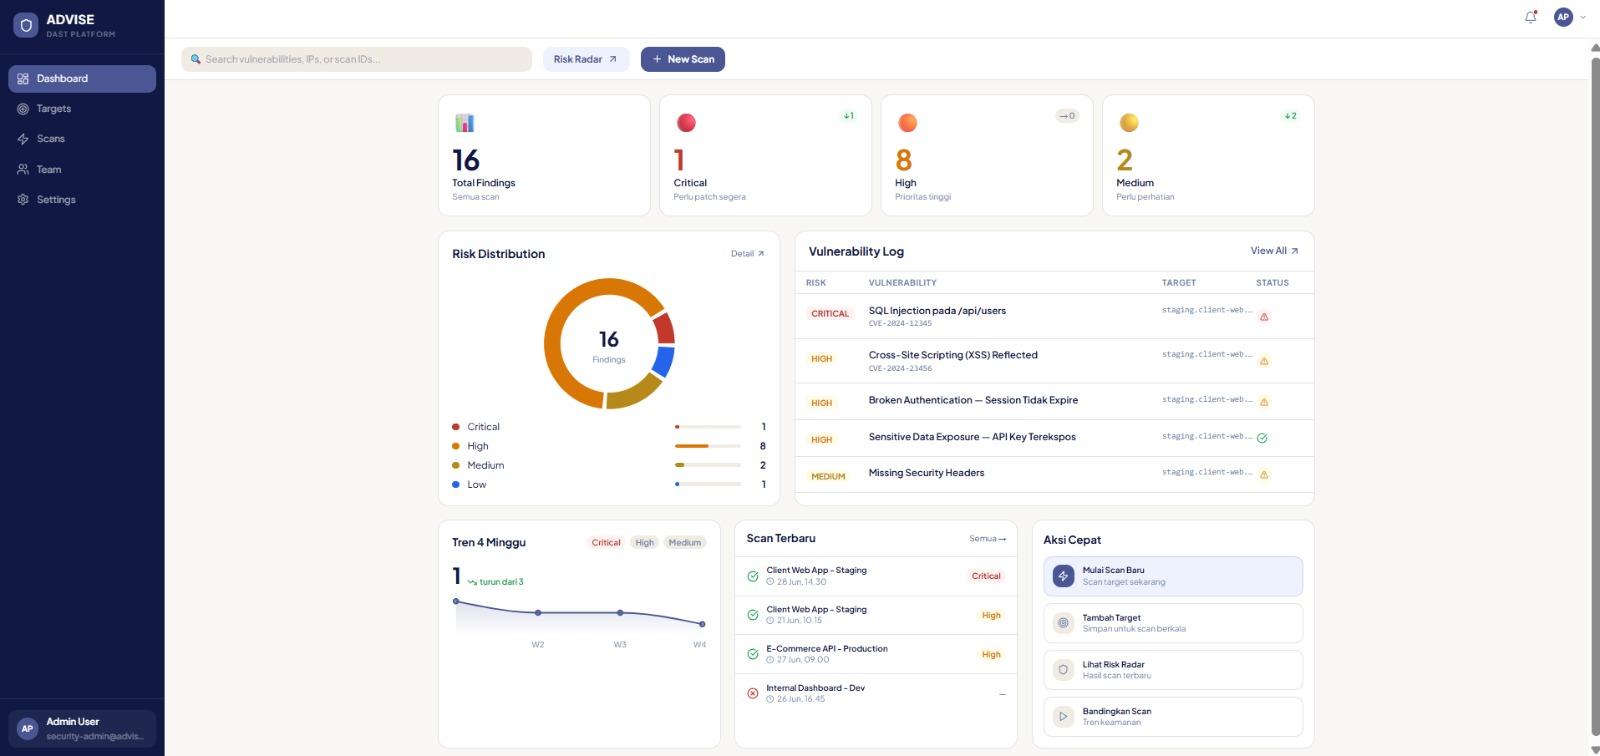
\includegraphics[width=0.95\linewidth]{dashboard.jpeg}
    \caption{Antarmuka Dashboard DAST "Advise"}
    \label{fig:dashboard}
\end{figure}

\subsection{Target (Manajemen Target)}
Fitur Target memungkinkan pengguna untuk mendaftarkan dan mengelola URL aplikasi web atau API yang akan menjadi target pemindaian. Pengguna dapat menambahkan target baru, mengonfigurasi autentikasi jika diperlukan, serta memvalidasi kepemilikan domain.
Alur kerjanya: Pengguna memasukkan URL target, sistem memvalidasi konektivitas, dan target tersebut kemudian tersedia untuk dipilih saat pengguna hendak memulai proses pemindaian baru. Desain ini dipilih untuk memudahkan pengelolaan banyak \textit{endpoint} secara terpusat.

\begin{figure}[H]
    \centering
    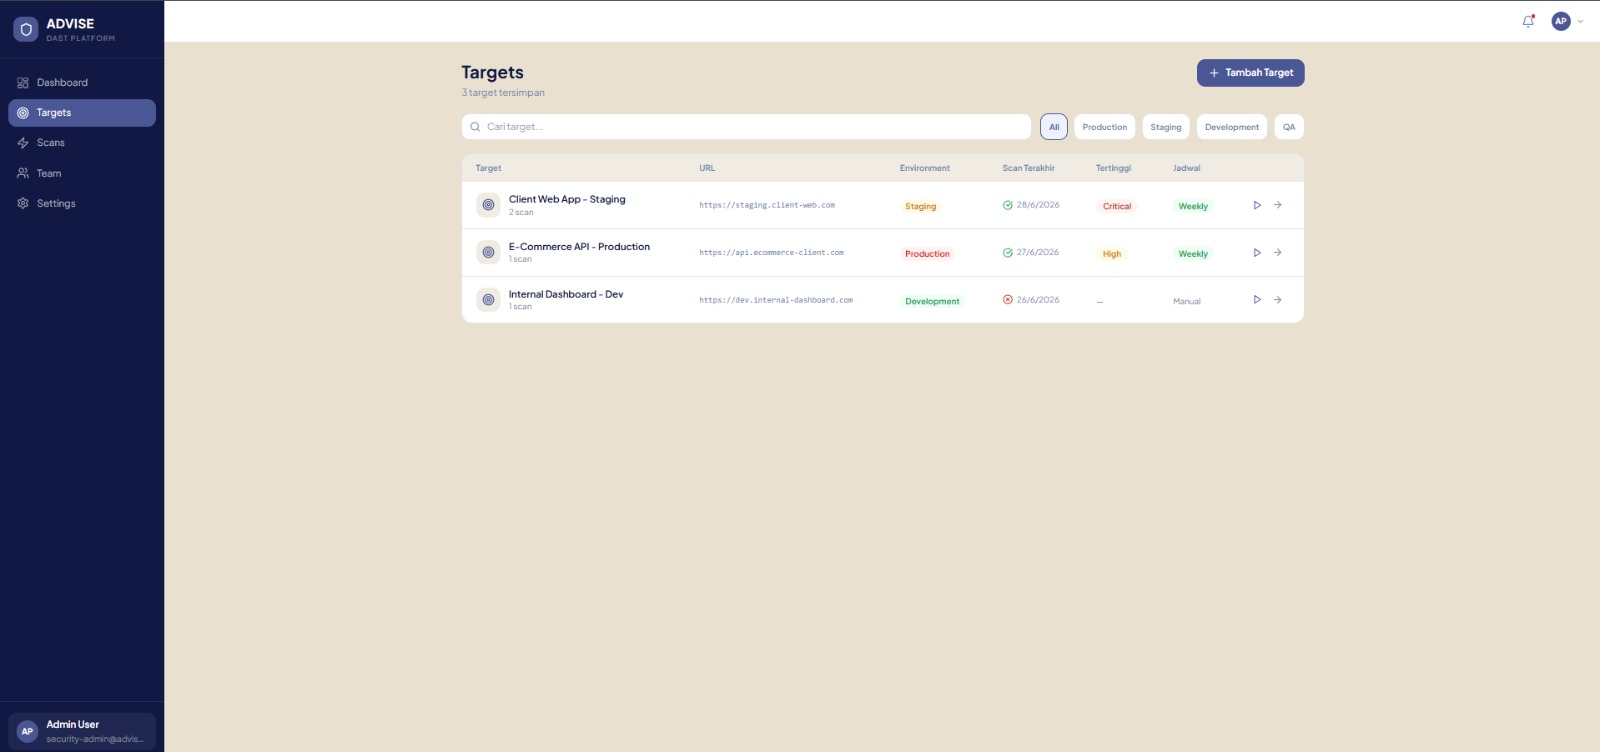
\includegraphics[width=0.95\linewidth]{target.jpeg}
    \caption{Antarmuka Manajemen Target}
    \label{fig:target}
\end{figure}

\subsection{Scans (Pemindaian)}
Fitur Scans adalah inti dari aplikasi ini, di mana pengguna dapat menginisiasi pemindaian keamanan baru, menjadwalkan pemindaian rutin, dan melihat riwayat pemindaian yang sedang atau telah berjalan. 
Cara kerjanya: Pengguna memilih target yang telah didaftarkan, menentukan profil pemindaian, dan memulai proses. Sistem akan mengeksekusi serangkaian \textit{payload} pengujian ke target untuk mencari celah keamanan. Pendekatan antarmuka ini dipilih untuk memisahkan konfigurasi pemindaian dengan eksekusi sehingga pengguna tidak bingung.

\begin{figure}[H]
    \centering
    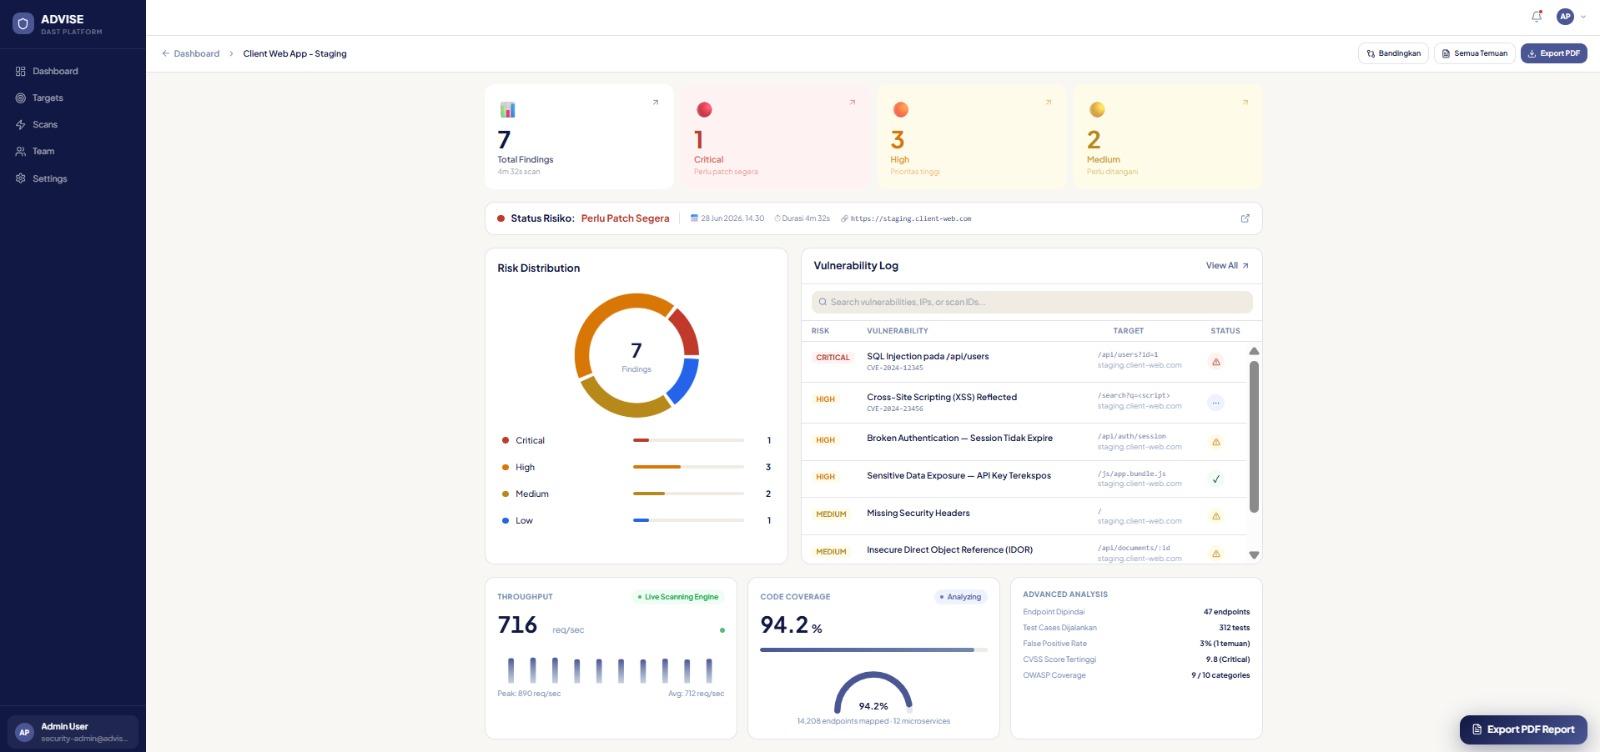
\includegraphics[width=0.95\linewidth]{scans.jpeg}
    \caption{Antarmuka Riwayat dan Konfigurasi Scans}
    \label{fig:scans}
\end{figure}

\subsection{Kerentanan (Vulnerabilities)}
Fitur Kerentanan menyajikan daftar lengkap kelemahan keamanan yang ditemukan dari hasil pemindaian. Setiap kerentanan diklasifikasikan berdasarkan tingkat keparahannya (Kritis, Tinggi, Sedang, Rendah).
Cara kerjanya: Saat pengguna mengklik salah satu kerentanan, sistem akan menampilkan detail teknis mengenai celah tersebut, letak URL yang rentan, serta saran remediasi (\textit{advise}) untuk memperbaikinya. Desain ini dirancang sedemikian rupa agar perbaikan dapat langsung dieksekusi oleh developer tanpa perlu mencari referensi luar.

\begin{figure}[H]
    \centering
    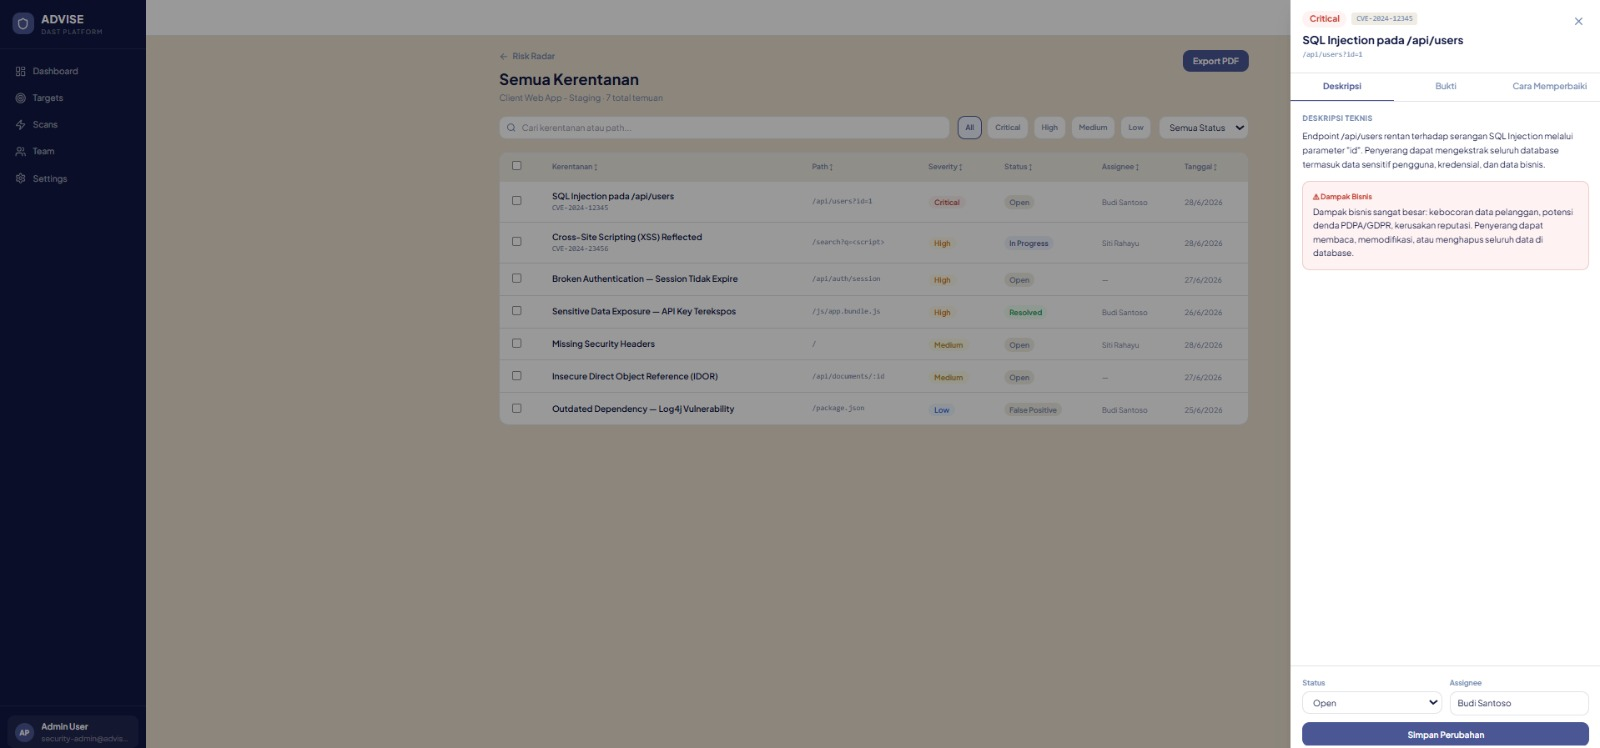
\includegraphics[width=0.95\linewidth]{kerentanan.jpeg}
    \caption{Antarmuka Daftar Kerentanan}
    \label{fig:kerentanan}
\end{figure}

\section{Analisis Urgensi}

Perancangan fitur-fitur pada aplikasi DAST "Advise" didasari oleh kebutuhan mendesak akan otomatisasi dan visibilitas dalam pengujian keamanan aplikasi. Berikut adalah alasan dan bagaimana fitur ini memberikan nilai tambah yang strategis bagi pengguna alat DAST:

\begin{itemize}
    \item \textbf{Visibilitas Menyeluruh}: Melalui Dashboard dan daftar Kerentanan yang terstruktur, tim keamanan dan \textit{developer} memiliki visibilitas langsung terhadap status keamanan seluruh aset digital mereka. Hal ini mengurangi waktu respons (\textit{Mean Time to Respond}) terhadap celah keamanan kritis.
    \item \textbf{Otomatisasi Pengujian}: Fitur Scans memungkinkan pemindaian dilakukan secara otomatis dan berkala, mengintegrasikan praktik \textit{Continuous Security} tanpa harus bergantung pada pengujian penetrasi manual yang memakan waktu dan biaya besar.
    \item \textbf{Rekomendasi yang Dapat Ditindaklanjuti (\textit{Actionable Advise})}: Nilai tambah terbesar dari alat DAST ini adalah pemberian saran perbaikan (\textit{remediation advice}) yang spesifik, sehingga developer dapat segera menambal celah tersebut, sesuai dengan filosofi nama "Advise".
    \item \textbf{Manajemen Terpusat}: Dengan adanya manajemen Target, pengguna yang mengelola banyak layanan (misalnya arsitektur \textit{microservices}) dapat mengawasi seluruh titik akhir dari satu antarmuka terpusat.
\end{itemize}

\section{Metodologi AI}

Dalam proses pemikiran, penyusunan arsitektur, dan penulisan kode fitur DAST "Advise", kami memanfaatkan bantuan AI untuk mempercepat siklus kerja. Berikut adalah penjelasan metodologi dan teknik \textit{prompting} yang diterapkan secara transparan:

\subsection{Ideasi dan Konseptualisasi}
Pada tahap awal, kami menggunakan model AI generatif untuk merancang ide tata letak dan struktur komponen (seperti terlampir pada gambar ideasi). Kami menggunakan percakapan berbasis \textit{chat} untuk mengklarifikasi kebutuhan pengguna dan memvisualisasikan arsitektur.

\textbf{Teknik Prompting}: Kami menerapkan teknik \textit{Role-Playing} dan memberikan konteks yang spesifik (\textit{Context-Setting}). 
\textit{Prompt}: "Bertindaklah sebagai UI/UX Designer untuk aplikasi keamanan siber. Rancang struktur komponen yang logis untuk halaman Dashboard DAST, dengan fokus menampilkan tingkat keparahan (severity) kerentanan dengan sangat jelas."

\begin{figure}[H]
    \centering
    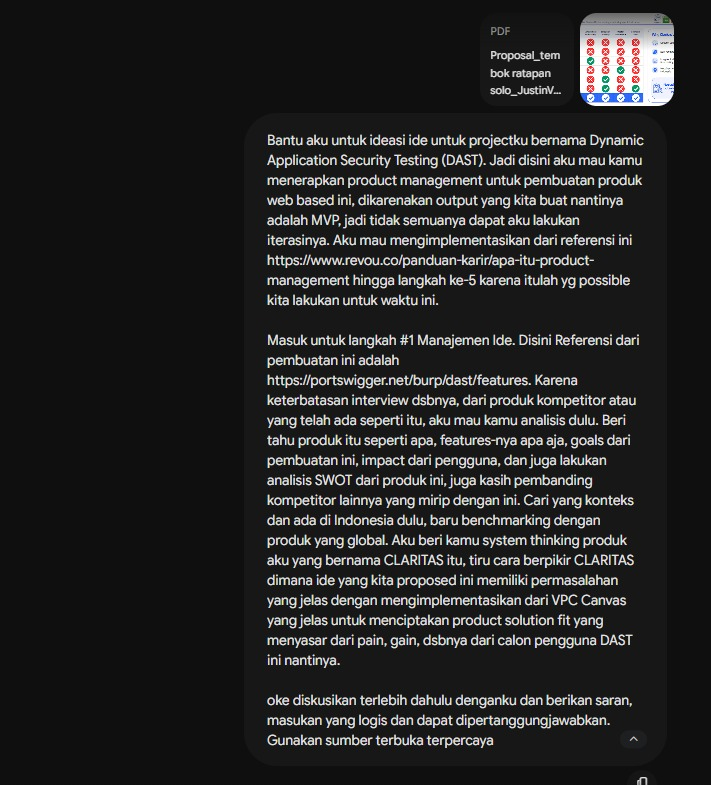
\includegraphics[width=0.95\linewidth]{ideasi.jpeg}
    \caption{Proses Ideasi Menggunakan Bantuan AI}
    \label{fig:ideasi}
\end{figure}

\subsection{Perancangan UI/UX}
Pada tahap selanjutnya, kami menggunakan \textit{prompt} komprehensif untuk merancang arsitektur informasi dan aliran UX untuk aplikasi DAST, yang kemudian dieksekusi dalam bentuk purwarupa Figma.

\textbf{Prompt yang Digunakan}:
\begin{quote}
\footnotesize
\textbf{Peran:} Bertindak sebagai Senior Product Designer untuk SaaS B2B.\\
\textbf{Produk:} ADVISE — DAST SaaS untuk software house, QA engineer, dan junior developer di Indonesia.\\
\textbf{Design tokens:} Primary \#111844, Secondary \#4B5694, Tertiary \#7288AE, Surface \#EAE0CF \& \#FFFFFF, semantic merah/oranye/kuning/biru muted untuk severity. Font Plus Jakarta Sans/Inter. Radius card 12px, button 8px.\\
\textbf{Instruksi:} Bangun base components dulu: Button, Input Field, Severity Badge, Data Table, Card, Side Drawer, Code Block, Toast — sebelum menyusun layar.\\
Susun 25 frame sesuai ID \& nama pada Bagian 3, dikelompokkan per modul (Onboarding, Core Scanning, Results \& Insights, Project Management, Team, Account/Billing, Edge States).\\
Untuk setiap frame, rujuk spesifikasi Komponen UI, States, dan Catatan Build Figma pada Bagian 4 sebagai requirement layout.\\
Pastikan navigasi antar frame memakai Figma prototyping link sesuai kolom Navigasi Lanjutan tiap layar, agar clickable prototype bisa diuji end-to-end mengikuti 3 user journey pada Bagian 5.\\
\textbf{Vibe akhir:} profesional B2B, minim friksi kognitif, ramah untuk developer junior — hindari ilustrasi terlalu playful atau warna terlalu jenuh.
\end{quote}

\subsection{Pembuatan Kode (\textit{Code Generation})}
Untuk implementasi \textit{frontend}, kami menggunakan asisten AI untuk membangun struktur kode Next.js dan styling dengan Tailwind CSS. Kode implementasi dan repositori proyek selengkapnya dapat diakses pada tautan berikut: \url{https://github.com/shzirley/DAST-netics-project}.

\textbf{Batasan (Constraints) yang Digunakan}: Kami memberikan \textit{constraints} tegas agar kode mematuhi standar produksi.
\textit{Prompt}: "Buat komponen React untuk menampilkan daftar kerentanan. Komponen harus menggunakan Tailwind CSS. Wajib menerima \textit{props} berupa array data kerentanan (id, nama, severity). \textbf{Constraint}: Gunakan \textit{client component} ('use client') dan pastikan desain \textit{responsive} untuk layar kecil dan besar."

\end{document}
